\documentclass[12pt,openright,oneside,a4paper,english,french,spanish]{abntex2}

\usepackage{cmap}	
\usepackage{lmodern}	
\usepackage[T1]{fontenc}	
\usepackage[utf8]{inputenc}		
\usepackage{lastpage}		
\usepackage{indentfirst}
\usepackage{color}	
\usepackage{graphicx}	
\usepackage{units}
\usepackage[brazilian,hyperpageref]{backref}
\usepackage[alf]{abntex2cite}
\usepackage{bold-extra}
\usepackage{eso-pic}
\usepackage{pdflscape}
\usepackage{tabu}
\usepackage{graphicx}
\usepackage[table,xcdraw]{xcolor}
\usepackage{multirow}
\usepackage{float}
\usepackage{xspace}
\usepackage[ruled,linesnumbered]{algorithm2e}
\usepackage{pdfpages}
\usepackage{caption}
\usepackage{graphicx}
% \usepackage{tabularx}
% \usepackage{booktabs}

\usepackage{booktabs,makecell,tabularx}
\usepackage{siunitx}
\usepackage{adjustbox}
\usepackage{array,booktabs}
\newcolumntype{C}[1]{>{\centering\arraybackslash}p{#1}}
\renewcommand\theadfont{\small}
\newcolumntype{L}{>{\raggedright\arraybackslash}X}

\newcommand{\itractool}{DTEST\xspace}

%Comandos para revisão
\newcommand{\rev}[1]{{\color{green}#1}\xspace}
\newcommand{\del}[1]{{\color{red}#1}\xspace}

%Comandos para impedir linhas órfãs e viúvas
\clubpenalty=10000
\widowpenalty=10000

\renewcommand{\backrefpagesname}{Citado na(s) página(s):~}
\renewcommand{\backref}{}
\renewcommand*{\backrefalt}[4]{
	\ifcase #1 %
		Nenhuma citação no texto.%
	\or
		Citado na página #2.%
	\else
		Citado #1 vezes nas páginas #2.%
	\fi}%
% ---


\usepackage{fixos/customizacoes}

% Dados pessoais
\autor{Igor Aragão Gomes}
\curso{Engenharia de Software}

% Dados do trabalho
\titulo{UNBIND: Uma ferramenta web para melhoria da qualidade de vida do estudante universitário}
\data{2023}
\palavraChaveUm{}
\palavraChaveDois{}

% Dados da orientacao
\orientador{Prof. Dr. Wander Cleber Pereira da Silva}

% Dados para a ficha catalográfica
\cdu{}

% Dados da aprovação do trabalho
\dataDaAprovacao{}
\membroConvidadoUm{}
\membroConvidadoDois{}

\local{Brasília, DF}
\instituicao{%
  Universidade de Brasília -- UnB
  \par
  Faculdade UnB Gama -- FGA
}
\tipotrabalho{Trabalho de Conclusão de Curso}
\preambulo{Monografia submetida ao curso de graduação em \imprimircurso\ 
da Universidade de Brasília, como requisito parcial para obtenção do Título 
de Bacharel em \imprimircurso.}

\definecolor{blue}{RGB}{41,5,195}
\makeatletter
\hypersetup{
     	%pagebackref=true,
		pdftitle={\@title}, 
		pdfauthor={\@author},
    	pdfsubject={\imprimirpreambulo},
	    pdfcreator={LaTeX with abnTeX2},
		pdfkeywords={abnt}{latex}{abntex}{abntex2}{trabalho acadêmico}, 
		colorlinks=true,       		% false: boxed links; true: colored links
    	linkcolor=blue,          	% color of internal links
    	citecolor=blue,        		% color of links to bibliography
    	filecolor=magenta,      		% color of file links
		urlcolor=blue,
		bookmarksdepth=4
}
\makeatother
\setlength{\parindent}{1.3cm}
\setlength{\parskip}{0.2cm}  
\makeindex


\begin{document}

\frenchspacing 
\imprimircapa
\imprimirfolhaderosto*

%\begin{fichacatalografica}
	\vspace*{\fill}					% Posição vertical
	\hrule							% Linha horizontal
	\begin{center}					% Minipage Centralizado
	\begin{minipage}[c]{12.5cm}		% Largura
	
	\imprimirautor
	
	\hspace{0.5cm} \imprimirtitulo  / \imprimirautor. --
	\imprimirlocal, \imprimirdata-
	\hspace{0.5cm} \pageref{LastPage} p. : il. (algumas color.) ; 30 cm.\\
	\hspace{0.5cm} \imprimirorientadorRotulo~\imprimirorientador\\
	Coorientador:\imprimircoorientador\\
	\hspace{0.5cm}
	\parbox[t]{\textwidth}{\imprimirtipotrabalho~--~\imprimirinstituicao,
	\imprimirdata.}\\
	\hspace{0.5cm}
		1. Aplicativos de Governo.
		2. Design da Experiência do Usuário.
		3. Desenvolvimento Orientado ao Comportamento.
		4. Transformação Digital.
		5. Teste caixa-preta.
		I. \imprimirorientador.
		II. \imprimircoorientador
		III. Universidade de Brasília.
		IV. Faculdade UnB Gama.
		V. \imprimirtitulo\\ 			
	
	\hspace{8.75cm} CDU \nomecdu\\
	
	\end{minipage}
	\end{center}
	\hrule
\end{fichacatalografica}

% \input{editaveis/errata}
\begin{folhadeaprovacao}

  \begin{center}
    {\ABNTEXchapterfont\large\imprimirautor}

    \vspace*{\fill}\vspace*{\fill}
    {\ABNTEXchapterfont\bfseries\Large\imprimirtitulo}
    \vspace*{\fill}

    \hspace{.45\textwidth}
    \begin{minipage}{.5\textwidth}
        \imprimirpreambulo
    \end{minipage}%
    \vspace*{\fill}
   \end{center}

   \begin{center}
    \vspace*{0.5cm}
    {\large\imprimirlocal}
    \par
    {\large\imprimirdata}
    \vspace*{1cm}
  \end{center}

\end{folhadeaprovacao}

%\input{editaveis/dedicatoria}
\begin{agradecimentos}


\end{agradecimentos}

\begin{epigrafe}
    \vspace*{\fill}
 	\begin{flushright}
		\textit{"Eu lhes disse essas coisas para que em mim vocês tenham paz. \\ 
		Neste mundo vocês terão aflições; contudo, tenham ânimo! Eu venci o mundo." \\
		(Bíblia Sagrada, João 16:33)}
	\end{flushright}
\end{epigrafe}

\begin{resumo}
Com o avanço da tecnologia, é possível observar também o aumento no grau de ansiedade e estresse nos estudantes universitários. É de suma importância a avaliação e o cuidado que o estudante universitário deve ter em relação à própria qualidade de vida. Com o propósito de auxiliar pessoas a terem uma avaliação pessoal em relação à própria vida, foi proposta a Roda da Vida. A pessoa que utiliza a ferramenta pode identificar, em três passos, as áreas da vida na qual está mais insatisfeita, podendo planejar ações e atividades para melhorar essa área. O objetivo deste trabalho é desenvolver uma ferramenta web que auxilie o estudante universitário a se avaliar a partir da Roda da Vida e receber recomendações de atividades que causem um impacto positivo em sua qualidade de vida. Para isso, foram empregados princípios da Revisão Sistemática de Literatura para análise de ferramentas semelhantes e um \textit{survey} para definição das atividades propostas.

 \vspace{\onelineskip}

 \noindent
 \textbf{Palavras-chave}: Qualidade de Vida. Roda da Vida. Engenharia de Software. Progressive Web App.
\end{resumo}

\begin{resumo}[Abstract]
 \begin{otherlanguage*}{english}


   \vspace{\onelineskip}

   \noindent
   \textbf{Key-words}: 
 \end{otherlanguage*}
\end{resumo}

\pdfbookmark[0]{\listfigurename}{lof}
\listoffigures*
\cleardoublepage
\pdfbookmark[0]{\listtablename}{lot}
\listoftables*
\cleardoublepage

\begin{siglas}

\item [UnB] Universidade de Brasília



\end{siglas}
\pdfbookmark[0]{\contentsname}{toc}
\tableofcontents*
\cleardoublepage


\textual

\chapter{Introdução}        
\label{ch:introducao}

    \section{Contexto}\label{contextualizacao}

O uso da tecnologia entre os estudantes universitários é destacadamente extenso, e tende a aumentar cada vez mais. Aproximadamente 80\% dos discentes das Instituições Federais de Ensino Superior Brasileiras indicam ter alguma ou muita experiência com computadores, enquanto 19,3\% dizem ter alguma noção e 1,3\% nenhuma noção. Em 2014, a IV Pesquisa havia registrado o percentual de 83,5\%. De todo modo, supera o patamar encontrado em 2010, quando o índice alcançou 78,0\% \cite{fonaprace2019}.

Ao mesmo tempo que se vê o avanço da tecnologia, se observa também o aumento na quantidade de estudos sobre a qualidade de vida dos graduandos, afinal, a mudança de rotina, do conteúdo que deve ser absorvido e do círculo de interações sociais, constituem uma nova fase na vida do ingresso em uma instituição de ensino superior. A rotina de estudos na universidade contribui para amplificar os problemas relativos à saúde mental, exigindo dos estudantes posturas flexíveis e resilientes no ambiente acadêmico \cite{fonaprace2019}.

Além disso, com a pandemia de COVID-19, estudos mostram que sete a cada dez universitários brasileiros tiveram um impacto negativo na sua saúde mental, e dentre esses, 87\% identificaram um aumento da ansiedade e do estresse \cite{chegg2021}.

Segundo a ONU, qualidade de vida é definida como a percepção do indivíduo sobre a sua posição na vida, no contexto da cultura e dos sistemas de valores nos quais ele vive, e em relação a seus objetivos, expectativas, padrões e preocupações \cite{whoqol1995}. Portanto, é possível perceber a importância da avaliação e do cuidado que o estudante universitário deve ter em relação à própria qualidade de vida.

Com o propósito de auxiliar pessoas a terem uma avaliação pessoal em relação à própria vida, foi proposta a ferramenta da Roda da Vida \cite{coachingtools}. Em três passos, ela propõe uma análise visual e crítica de como estão certas áreas da vida de quem a utiliza. O primeiro passo consiste em definir áreas relevantes da própria vida. O próximo é avaliar o quanto a pessoa está satisfeita com cada uma das categorias definidas. Assim, a pessoa que está se avaliando, pode finalizar com o último passo, que é traçar um plano de ações ou atividades que possam ser realizadas no intuito de melhorar a qualidade de vida.
    
    \section{Revisão Bibliográfica}

Existem diversos instrumentos desenvolvidos para avaliar qualidade de vida. Os instrumentos mais utilizados para tal são o WHOQOL-100, e também sua versão abreviada, WHOQOL-BREF, ambos sugeridos pela OMS. O WHOQOL-100 é composto por 100 itens, divididos em 24 subdomínios, que são distribuídos entre seis domínios (físico, psicológico, nível de independência, relações sociais, meio ambiente e religiosidade ou espiritualidade) \cite{whoqol1995}.
Já o WHOQOL-BREF possui 26 itens, e os mesmos 24 subdomínios, que desta vez são distribuídos entre quatro domínios (físico, psicológico, relações sociais e meio ambiente) \cite{whoqol1995}. Essas ferramentas são utilizadas para estudos epidemiológicos com o objetivo de avaliar e planejar sistemas de saúde, e são as mais empregadas em pesquisas sociais \cite{gorenstein2015}.

Outro instrumento de medição de qualidade de vida é o Questionário Genérico de Qualidade de Vida SF-36 que foi desenvolvido especificamente para pesquisas em saúde. Ele fornece um perfil funcional da saúde e do bem-estar do indivíduo, bem como um escore global de suas saúdes física e mental. É um questionário abrangente que pode ser utilizado em qualquer idade e doença, assim como em populações saudáveis \cite{gorenstein2015}. Contudo, sua aplicação se torna inviável a este trabalho pela falta de inclusão de categorias relativas a adequação do sono, funcionamento cognitivo e sexual, funcionamento familiar, autoestima, alimentação, recreação, hobbies, comunicação e sintomas e problemas específicos \cite{gorenstein2015}.

Nota-se que o foco dos instrumentos SF-36, WHOQOL-100 e suas variações, é avaliar a qualidade de vida de um público geral para utilização em estudos populacionais. Pela dinâmica proposta neste trabalho, onde o público alvo são os estudantes universitários, utilizaremos outra ferramenta, a Roda da Vida.


    
    \section{Problema}

Existem diversas ferramentas e plataformas que buscam auxiliar a qualidade de vida do usuário. Porém, os softwares gratuitos que têm saúde mental e qualidade de vida como foco dispõem de poucas funcionalidades, enquanto os softwares pagos podem não ser acessíveis para estudantes que possuem baixa renda.

Sabendo disso, a pergunta de pesquisa definida neste trabalho é:

“Como desenvolver uma ferramenta web gratuita que contribua para a melhoria da qualidade de vida dos estudantes acadêmicos tendo como base os princípios e passos da Roda da Vida?”

    \section{Objetivos}
\subsection{Objetivo Geral}

O objetivo geral deste trabalho é desenvolver uma ferramenta web que auxilia estudantes acadêmicos a melhorar a qualidade de vida.

A ferramenta irá implementar um questionário com perguntas avaliativas sobre diversas áreas de sua vida, e irá gerar um diagrama com a pontuação para cada uma das categorias da Roda da Vida. Após a análise do diagrama, o sistema irá sugerir atividades que possam influenciar positivamente nas áreas da vida que o usuário obteve menor pontuação.

\subsection{Objetivos Específicos}
\begin{itemize}
    \item Analisar estrutura da Roda da Vida
    \item Analisar ferramentas semelhantes à proposta neste trabalho
    \item Definir áreas da vida relevantes na vida do estudante acadêmico
    \item Definir lista de atividades que auxiliem na qualidade de vida do estudante acadêmico
    \item Definir a arquitetura e desenho do software
    \item Definir o método de desenvolvimento do sistema
    \item Desenvolver o sistema
\end{itemize}

    \section{Metodologia}

Este capítulo aborda a metodologia de trabalho adotada para o desenvolvimento do projeto, desde a definição do tema até a conclusão dos objetivos propostos. Ela é baseada no modelo Cascata \cite{royce1987managing}, onde há uma correlação entre cada fase, e todo o processo é planejado antes de sua execução. A Figura \ref{fig:metodologia-simples} é uma representação gráfica da metodologia abordada.

\begin{figure}[H]
\centering
\caption{Metodologia abordada no projeto}
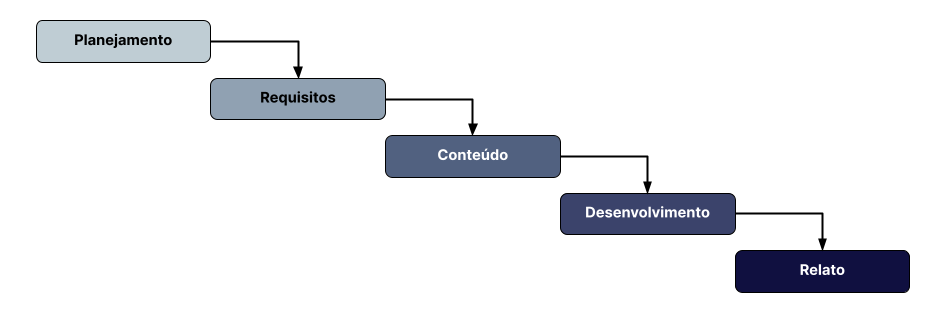
\includegraphics[width=1\textwidth]{figuras/imagens/metodologia-simples.png}
\legend {(Fonte: Elaborado pelo Autor)}
\label{fig:metodologia-simples}
\end{figure}



    \section{Organização do Trabalho}

Este trabalho de conclusão de curso está organizado nos seguintes capítulos:

\begin{itemize}

 \item \textbf{Capítulo \ref{ch:introducao} - Introdução:} neste capítulo foram apresentados o contexto do trabalho,  o problema de pesquisa, os objetivos deste trabalho e, uma síntese da metodologia planejada;
 
    \item \textbf{Capítulo \ref{ch:referencial} - Referencial teórico:} descreve os conceitos que fundamentam este trabalho. O capítulo é subdividido nas seções...
    
     \item \textbf{Capítulo \ref{ch:metodologia} - Materiais e Métodos:} apresenta o plano metodológico adotado de forma mais detalhada e caracteriza o objeto de estudo;
     
     \item \textbf{Capítulo \ref{ch:proposta} - Proposta:} Apresenta a proposta deste trabalho, desde a abordagem até a proposta de um módulo para a ferramenta de suporte ao processo de transformação digital do governo brasileiro.

\end{itemize}

\chapter{Referencial Teórico}
\label{ch:referencial}

\section{Considerações Iniciais}
Neste capítulo é apresentado o referencial teórico, o qual foi realizada por meio de uma
revisão de literatura...

%---------------- UXD ---------------------%
\section {Referencial Teórico 1}






\section{Referencial Teórico 2}





\section{Referencial Teórico 3}


\section{Considerações Finais}



%     \chapter{Proposta do Trabalho}
\label{ch:proposta}

\section{Considerações Iniciais}

Neste capítulo é retomado o plano metodológico apresentado brevemente no Capítulo \ref{ch:metodologia} e apresenta um detalhamento da proposta deste trabalho bem como as atividades já realizadas e as atividades a serem realizadas... 

\section{Planejamento de Pesquisa}

Nesta fase foram definidos o tema de pesquisa, a questão de pesquisa, o objetivo a ser atingido e a classificação metodológica. O Capítulo \ref{ch:introducao} contempla esta fase.

\section{Coleta de Dados}

Nesta fase foram adotadas técnicas como Pesquisa Bibliográfica e \textit{Design Science Research} para a coleta de dados. 

\subsection{Pesquisa Bibliográfica}

\section{Cronograma}

\chapter{Materiais e Métodos}
\label{ch:metodologia}
\section{Considerações Iniciais}

Neste capítulo apresenta-se o plano metodológico adotado para alcançar o objetivo desta pesquisa, isto é...

\section{Plano Metodológico}

O plano metodológico adotado possui 4 fases: Planejamento de pesquisa; Coleta de dados; Análise de dados; e Resultados...


\subsection{Planejamento} Nesta fase foram definidos o tema de pesquisa, a questão de pesquisa, o objetivo a ser atingido e a classificação metodológica.

\subsection{Coleta de Dados} Nesta fase foram adotadas técnicas como \textit{Pesquisa Bibliográfica} e \textit{Design Science Research} para a coleta de dados...

\subsection{Analise de Dados} Nesta fase é feita uma analise nos resultados observados nas fases anteriores.

\subsection{Resultados} Esta fase corresponde à fase final deste trabalho, na qual os resultados obtidos com a execução do Trabalho de Conclusão 2 serão apresentados. 

\section{Considerações Finais}

Neste capítulo, foi apresentado o plano metodológico adotado para se atingir os objetivos desta pesquisa. No próximo capítulo apresenta-se a proposta deste trabalho, com as atividades já realizadas e as que ainda serão realizadas. 
    \chapter{Proposta do Trabalho}
\label{ch:proposta}

\section{Considerações Iniciais}

Neste capítulo é retomado o plano metodológico apresentado brevemente no Capítulo \ref{ch:metodologia} e apresenta um detalhamento da proposta deste trabalho bem como as atividades já realizadas e as atividades a serem realizadas... 

\section{Planejamento de Pesquisa}

Nesta fase foram definidos o tema de pesquisa, a questão de pesquisa, o objetivo a ser atingido e a classificação metodológica. O Capítulo \ref{ch:introducao} contempla esta fase.

\section{Coleta de Dados}

Nesta fase foram adotadas técnicas como Pesquisa Bibliográfica e \textit{Design Science Research} para a coleta de dados. 

\subsection{Pesquisa Bibliográfica}

\section{Cronograma}


\bookmarksetup{startatroot} 

\postextual

\bibliography{bibliografia} 
%\begin{anexosenv}
\partanexos

\end{anexosenv}


\begin{apendicesenv}

\partapendices

\end{apendicesenv}

\printindex
\end{document}

